\documentclass[11pt]{article}
\usepackage[utf8]{inputenc}
\usepackage[portuguese]{babel}
\usepackage{helvet}
\usepackage[helvet]{sfmath}
\everymath={\sf}
\usepackage[T1]{fontenc}
\usepackage[a4paper, left=3cm, top=3cm, right=2.5cm, bottom=3cm]{geometry}
\usepackage{setspace}
\usepackage[hang]{footmisc}
\usepackage{cite}
\usepackage{titlesec}
\usepackage{subfiles}
\usepackage[cache=false]{minted}
\usepackage{enumitem}
\usepackage{csquotes}
\usepackage{url}
\usepackage{hyperref}
\usepackage{graphicx}
\usepackage{pdfpages}
\usepackage[font=footnotesize]{caption}
\hypersetup{
    colorlinks,
    citecolor=black,
    filecolor=black,
    linkcolor=black,
    urlcolor=black
}
\setstretch{1.5}
\setminted{
    fontsize=\footnotesize,
    linenos=true
}
\renewcommand\familydefault{\sfdefault}
\titleformat{\subsection}%
{\normalfont\large}{\hspace*{\parindent}\thesubsection}{1em}{\hrulefill\hspace*{2pt}\raisebox{-.1\ht\strutbox}}

\newenvironment{performex}{\begin{displayquote}\itshape\setstretch{1.2}}{\end{displayquote}}

\newcommand{\Section}[1]{\clearpage\phantomsection\addcontentsline{toc}{section}{#1}\section*{#1}}
\newcommand{\Subsection}[1]{\phantomsection\addcontentsline{toc}{subsection}{#1}\subsection*{#1}}
\newcommand{\Subsubsection}[1]{\phantomsection\addcontentsline{toc}{subsubsection}{#1}\subsubsection*{#1}}
\newcommand{\Subsubsubsection}[2]{\phantomsection\begin{itemize}\item[#1.]\textsl{#2}\end{itemize}}

\newcommand{\bkitem}[1]{\item[\textbf{#1:}]}

\begin{document}

\tableofcontents

\Section{Introdução}
\subfile{Chapters/intro.tex}

\Section{Contextualização Teórica}
\subfile{Chapters/state_of_art.tex}

\Section{Linguagem Performática da Música}
\subfile{Chapters/concepts.tex}

\Section{Análise da Obra}
\subfile{Chapters/obra.tex}

\Section{Discussão e Considerações Finais}
\subfile{Chapters/discussion.tex}

\clearpage\phantomsection\addcontentsline{toc}{section}{Referências}
\bibliography{bibthesis}
\bibliographystyle{unsrt}

\Section{Anexos}
\section*{Anexo I - Código para a plataforma Web}
\subfile{Chapters/code.tex}

\section*{Anexo II - Partitura da Obra}
Link para suporte auditivo da obra:

{\footnotesize
\url{https://drive.google.com/drive/folders/1Y0O9PNRTglBG0XmN7_A9dn7ZV3kqV4je?usp=share_link}}

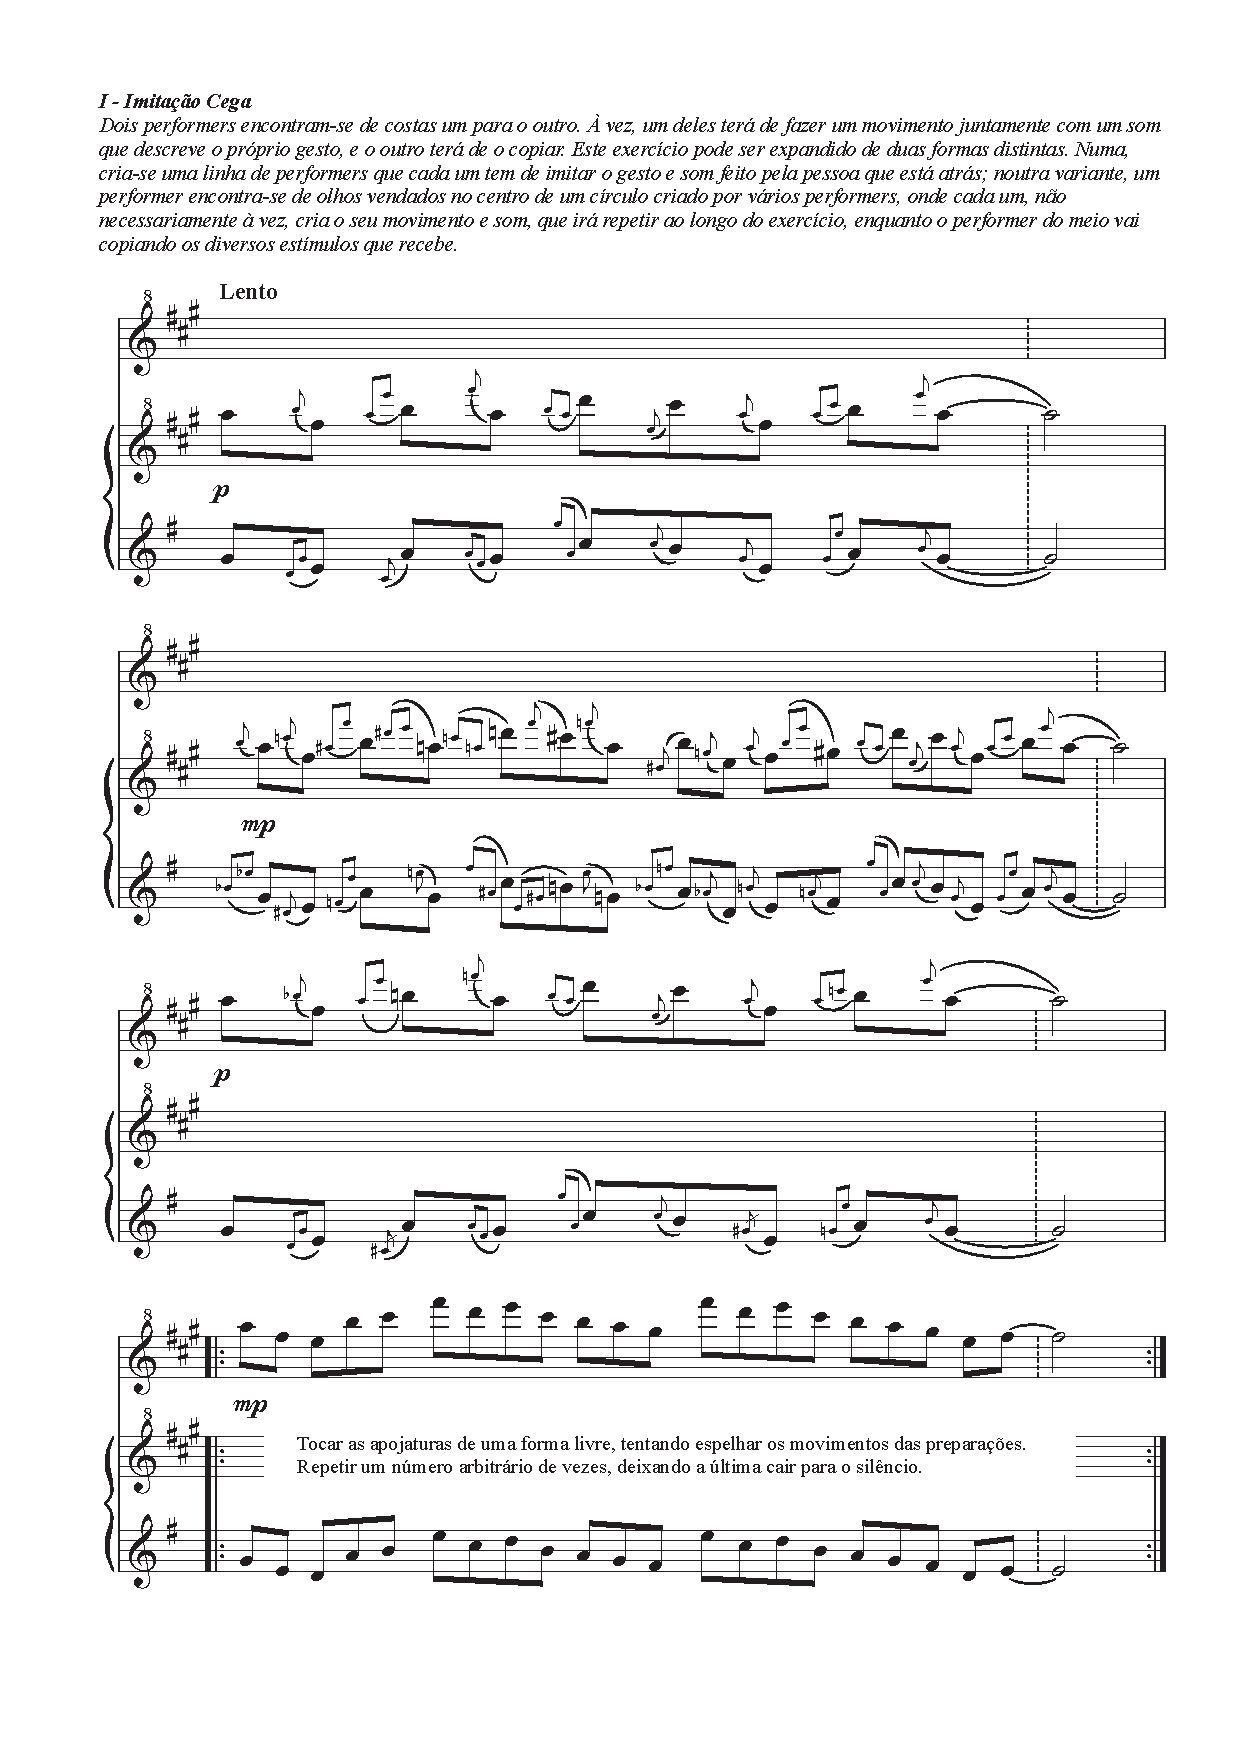
\includepdf[pages=-]{../music/obra.pdf}

\end{document}